%!TEX root = ../terrainbook.tex
% chktex-file 46

\setchapterpreamble[u]{\margintoc}
\graphicspath{{topofeatures/}}


\chapter{Topographic properties and features}%
\label{chap:topofeatures}

While a terrain is a (2.5D) surface, it can also be conceptualised as an aggregation of many \emph{topographic features} that are inter-related.%
\index{topographic feature}
Common examples of features are peaks, ridges, valleys, lakes, cliffs, etc., but one can think of application-specific ones such as the navigational channels in bathymetry, buildings in city modelling, or dikes for flood modelling.

Identifying the different features forming a terrain enhances our understanding of the raw dataset.
To help us extract and identify features, some properties (or characteristics) need to be extracted from terrains.

We describe in this chapter the main properties of terrains, explain how they can be extracted, and how they are used in practice (for specific use-cases in different fields, and to identify features).



%%%
%
\section{Topographic properties}%
\label{sec:topoproperties}

We describe in this section the main topographic properties that are commonly extracted from terrains:
\begin{itemize}
  \item slope
  \item curvature
  \item roughness
\end{itemize}

Since these differ significantly from the data model used (TINs and grids), we give examples for both.

%%%
\paragraph{For grids.}
The extraction of these properties is more common with grids, and in most cases kernel filters are used, Figure~\ref{fig:filter} shows one example.
\begin{marginfigure}
  \centering
  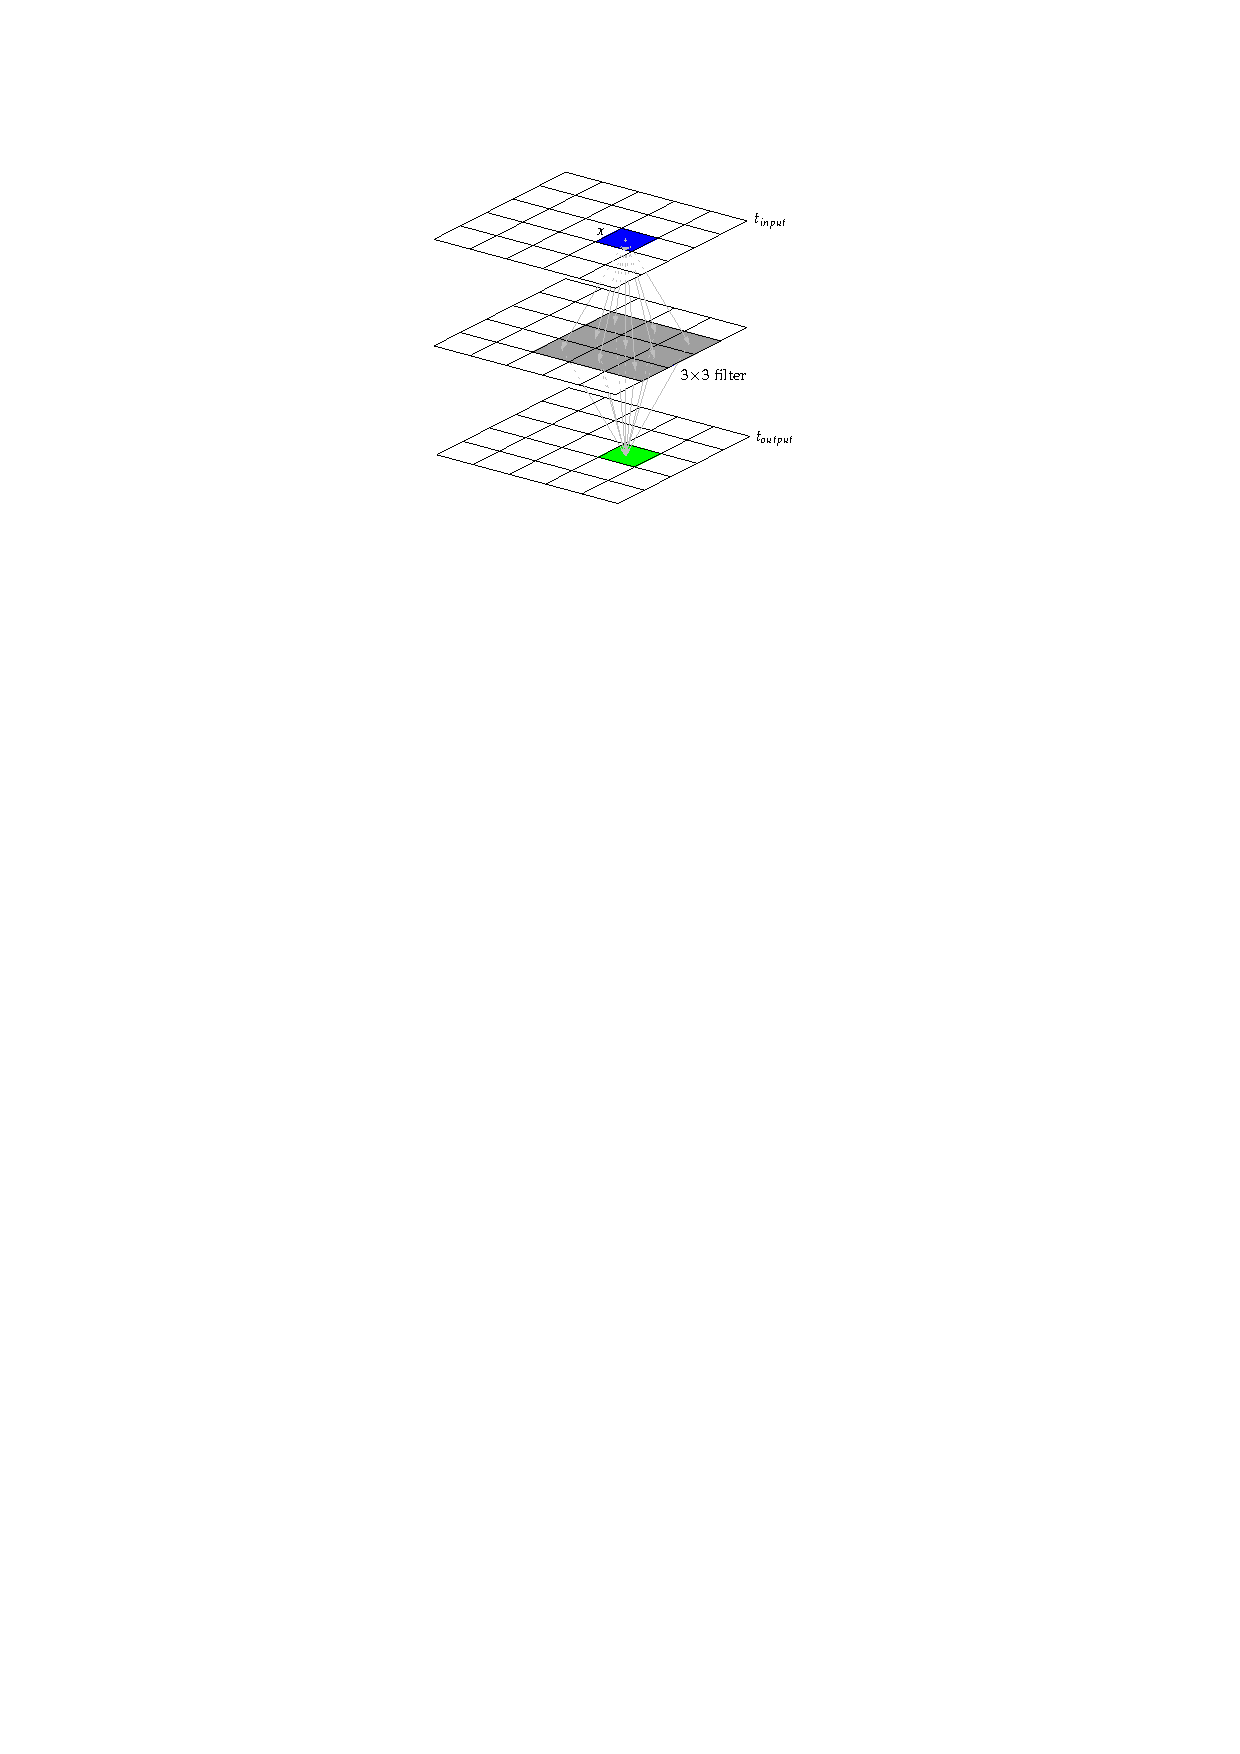
\includegraphics[width=\linewidth]{figs/filter}
  \caption{Example of a 3$\times$3 filter. The new value of the cell $x$ of the input (in blue) is calculated by using its 8 neighbours (\eg\ averaging the values) and the output terrain $t_{output}$ contains that value for its cell $x$. This operation is usually performed for all cells in the input $t_{input}$.}%
\label{fig:filter}
\end{marginfigure}%
\index{kernel filter}
A filter is conceptually the same as a focal operation in map algebra (in GIS), as as a convolutional filter in computer vision.
Observe that in Figure~\ref{fig:filter} a 3$\times$3 window is shown, but a 5$\times$5%
% \marginnote{5$\times$5 filters can be used}
or larger window could also be used; the size to use depends on the scale at which one wants to extract a property.
The main advantage of grids is that the value of a property can be easily calculated and the output is a new grid having the same resolution and orientation, but the values are the property (\eg\ the gradient at this location) instead of the elevation.

%%%
\paragraph{For TINs.}
A given property is in most cases as easy as for a grid to calculate for a given location ($x,y$), but the issue is how to store the results: in a grid? only a set of points?
This makes the use of TINs more cumbersome in practice.



%%%
%
\subsection{Slope}%
\index{slope}

\begin{figure}
  \centering
  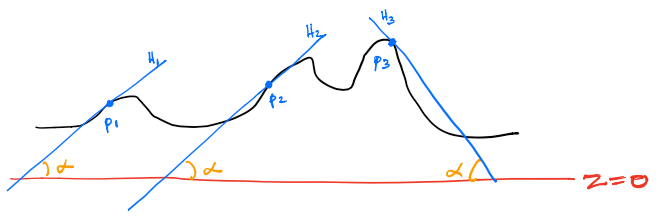
\includegraphics[width=\linewidth]{figs/slope_concept}
  \caption{The slope at a given location $p_i$ is defined by the tangent plane $H_i$ to the surface. Here are 3 examples for a profile view of a terrain.}%
\label{fig:slope_concept}
\end{figure}

The slope at a given location $p$ on a terrain is defined by the plane $H$ that is tangent at $p$ to the surface representing the terrain (see Figure~\ref{fig:slope_concept}).
What we casually refer to as `slope' has actually two components (see Figure~\ref{fig:slope_aspect}).%: 
\begin{enumerate}
  \item gradient 
  \item aspect 
\end{enumerate}
\marginnote{slope has 2 components: gradient + aspect}
\begin{figure}
  \centering
  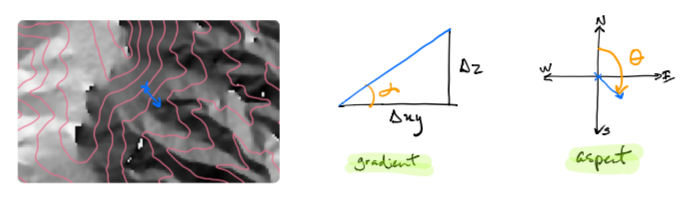
\includegraphics[width=\linewidth]{figs/slope_aspect}
  \caption{One DTM with contour lines, and the gradient and aspects concepts for a given location (blue cross).}%
\label{fig:slope_aspect}
\end{figure}


%%%
\paragraph{Gradient.} 
The gradient at a given point $p$ is the maximum rate of change in elevation. 
It is obtained by the angle $\alpha$ between $H$ and the horizontal plane (Figure~\ref{fig:slope_aspect}).
From a mathematical point-of-view, the gradient is the maximum value of the derivative at a point on the surface of the terrain (maximised over the direction).
The gradient will often be expressed in degrees, or in percentage.

Notice that if we calculate the gradient at every location for a terrain, then we obtain a new field since the gradient is a continuous phenomena (values from 0\% to 100\% for instance).
This means in practice that for a given terrain in raster, calculating its gradient will create a new raster file that can be further processed.


%%%
\paragraph{Aspect.}
At a given point $p$ on the terrain the gradient can be in any direction, the aspect is this direction projected to the $xy$-plane. 
It is basically a 2D vector telling us the direction of the steepest slope at a given point.
It is usually expressed in degrees from an arbitrary direction (most often the north).
Observe that for the parts of the terrain that are horizontal (\eg\ a lake) the value of the aspect is unknown.
Also observe that at a given location the aspect will always be perpendicular to the contour line.


% GDAL: % https://www.gdal.org/gdaldem.html#gdaldem_aspect
% values between 0° and 360° representing the azimuth that slopes are facing. The definition of the azimuth is such that : 0° means that the slope is facing the North, 90° it's facing the East, 180° it's facing the South and 270° it's facing the West (provided that the top of your input raster is north oriented).



%%%
\paragraph{Slope in TINs.}

Calculating the slope in a TIN is fairly straightforward: for a point $p=(x,y)$ find the triangle $\tau$ containing this point, and compute the normal vector $\vec{n}$ of $\tau$ (pointing outwards). 
The projection of $\vec{n}$ on the $xy$-plane is the aspect (this is done by simply ignore the $z$-component of the vector).
And the gradient is obtained easily.

If $p$ is directly on a edge of the TIN then the solution cannot be obtained directly; it is common practice to calculate the normal vector of the 2 incident triangle and average them to obtain one $\vec{n}$.
The same is applied if $p$ is directly on a vertex $v$ of the TIN: the average of all the normal vectors of all the incident triangle to $v$ is used.


%%%
\paragraph{Slope in grids.}

If the terrain is represented as a regular grid (say of resolution $r$), then there exist several algorithm to obtain the slope at a given cell $c_{i,j}$.
We list here a few common ones.
It should be noticed that most algorithms use a 3$\times$3 kernel, \ie\ the value for the gradient/aspect at cell $c_{i,j}$ is computed by using (a subset of) the 8 neighbours.
\begin{marginfigure}
  \centering
  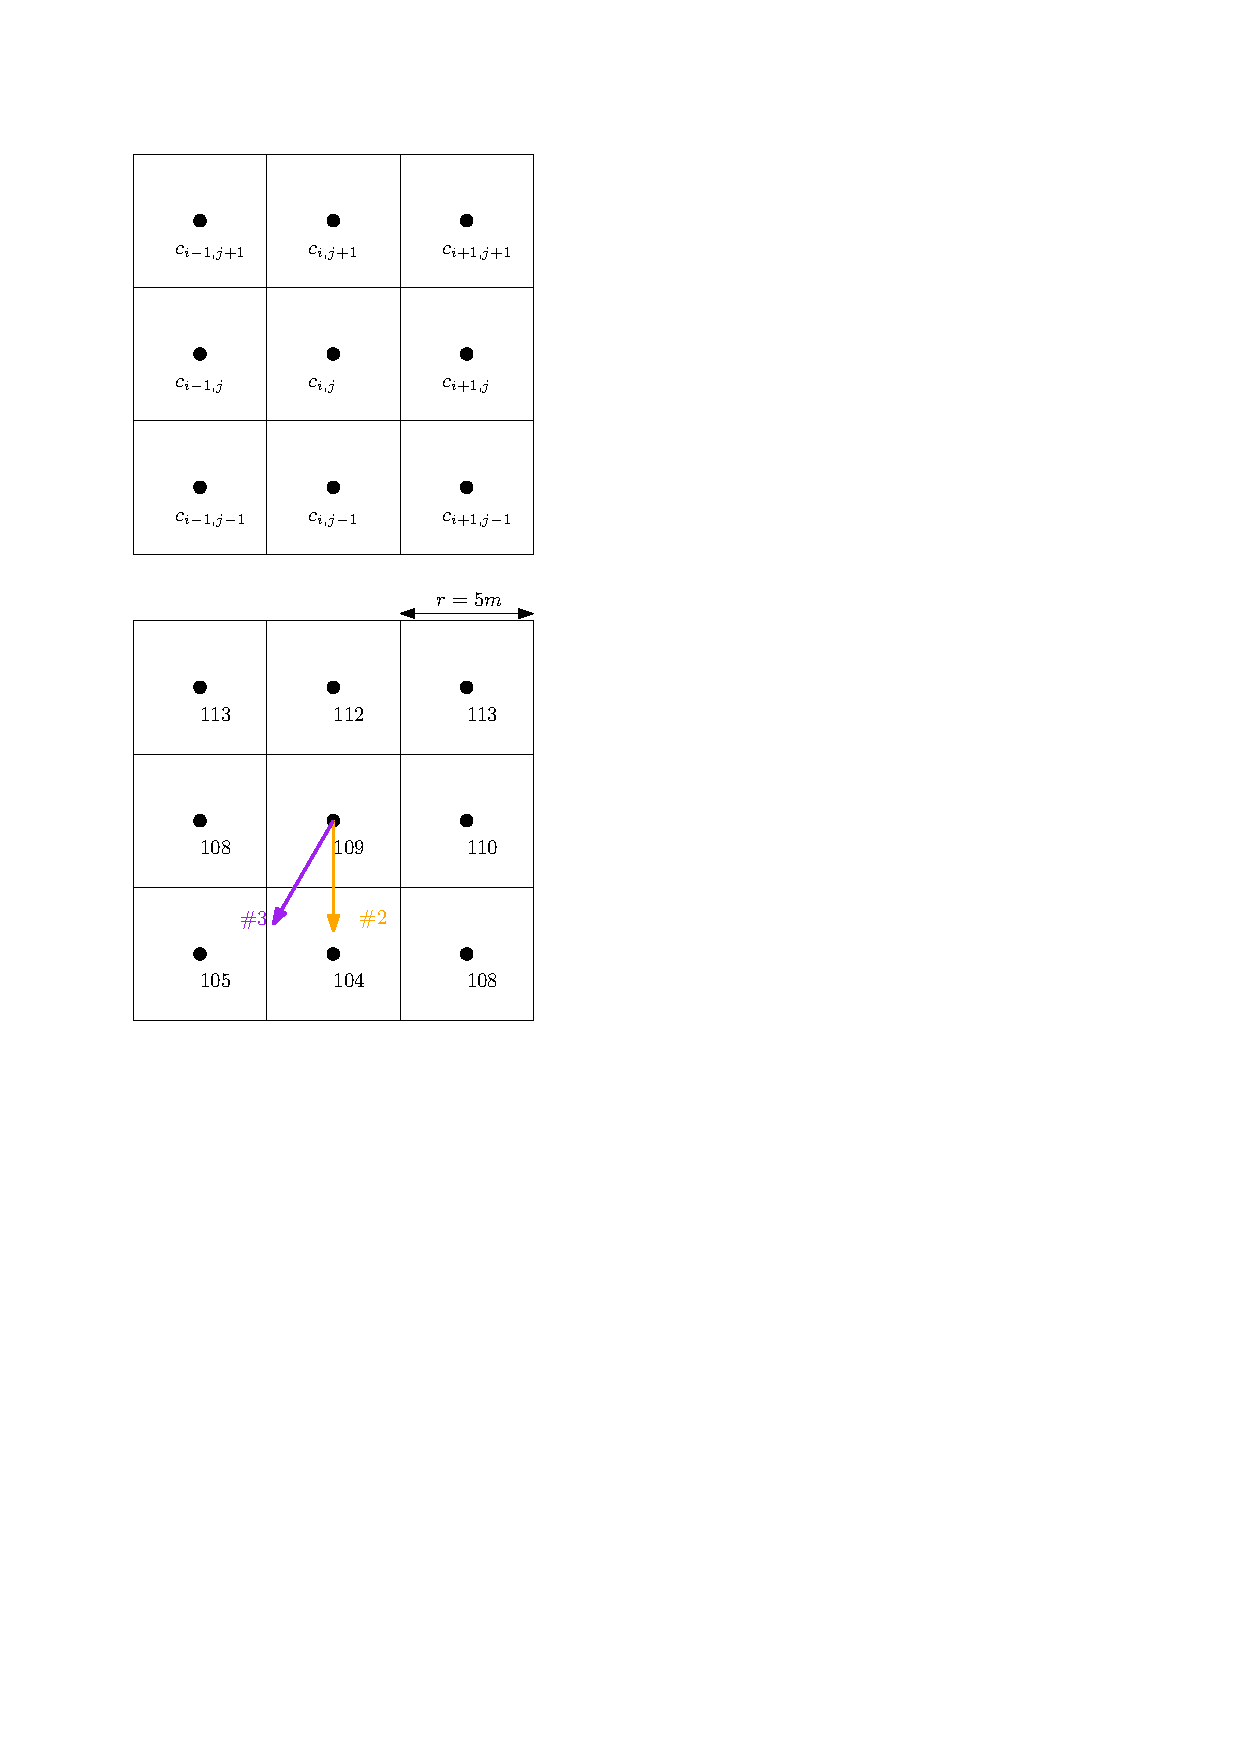
\includegraphics[width=\linewidth]{figs/slope_grid}
  \caption{\textbf{(top)} Given a cell $c_{i,j}$, the 3$\times$3 kernel and its 8 neighbours. \textbf{(bottom)} A hypothetical case with some elevations; orange = aspect for method \#2 below, purple = aspect for method \#3 below.}%
\label{fig:slope_grid}
\end{marginfigure}


%%%
\paragraph{1. Local triangulation + TIN method.}
It is possible to locally triangulate the 9 points, calculate the normal of the 8 triangles, and then use the method above for TINs.


%%%
\paragraph{2. Maximum height difference.}
This method simply picks the maximum height difference between $c_{i,j}$ and each of its 8 neighbours, the maximum absolute value is the direction of the aspect and the gradient can be trivially calculated.
Notice that this means that there are only 8 possibilities for the slope (at 45\degree\ intervals).
For the case in Figure~\ref{fig:slope_grid}, the aspect would be facing south (180\degree) and the gradient would be 45\degree.


%%%
\paragraph{3. Finite difference.}

With this method, the height differences in the $x$-direction (west-east) and in the $y$-direction (south-north) are calculated separately, and then the 2 differences are combined to obtain the slope.
This means that only the direct 4-neighbours of $c_{i,j}$ are used.

\begin{equation}
  \frac{\partial z}{\partial x} = \frac{z_{i-1,j} - z_{i+1,j}}{2\,r}
\, , 
  \frac{\partial z}{\partial y} = \frac{z_{i,j-1} - z_{i,j+1}}{2\,r}
\end{equation}

The gradient is defined as:
\begin{equation}
  \tan \alpha = \sqrt{(\frac{\partial z}{\partial x})^2 + (\frac{\partial z}{\partial y})^2}
\end{equation}

and the aspect as:
\begin{equation}
  \tan \theta = \frac{\frac{\partial z}{\partial y}}{\frac{\partial z}{\partial x}}
\end{equation}

The value of $\theta$ should be resolved for the correct trigonometric quadrant, and if $\frac{\partial z}{\partial x} = 0$ then it means the aspect should be handled differently (considering only the variation in the south-north direction). 

For the case in Figure~\ref{fig:slope_grid}, the gradient would be 39.5\degree\ and the aspect would be 194.0\degree.


%%%
\paragraph{4. Local polynomial fitting.}%
\label{sec:polynomial}

Based on the 9 elevation points, it is possible to fit a polynomial (as explained in Chapter~\ref{chap:interpol}) that approximate the surface locally; notice that the polynomial might not pass through the point if a low-degree function is used.

A quadratic polynomial could for instance be defined:
\begin{equation}
  f(x,y) = ax^2 + by^2 + cxy + dx + ey +d
\end{equation}
, and thus:
\begin{equation}
  \frac{\partial f}{\partial x} = 2ax + cy + d
\end{equation}
\begin{equation}
  \frac{\partial f}{\partial y} = 2by + cx + e
\end{equation}
and if a local coordinate system centered at $c_{i,j}$ is used, then $x = y = 0$, and thus $\frac{\partial f}{\partial x} = d$ and $\frac{\partial f}{\partial y} = e$.


\begin{floatbox}
  \begin{kaobox-practice}[frametitle=\faCog\ How does it work in practice?]
    The GDAL utility \texttt{gdaldem} (\url{https://www.gdal.org/gdaldem.html}) does not have the best documentation and does not explicitly mention which method is used.

    After some searching, we can conclude that the method ``4. Local polynomial fitting'' is used by default for slope/aspect, and specifically the Horn's method is used~\citep{Horn81}.
    This uses a 3$\times$3 window, and fits a polynomial; the centre pixel value is not used.

    If the option \texttt{-alg ZevenbergenThorne} is used, then the algorithm of \citet{Zevenbergen87} is used. 
    This uses only the 4 neighbours, and is a variation of the method ``3. Finite difference'' above.

    The documentation of \texttt{gdaldem} states that: ``literature suggests Zevenbergen \& Thorne to be more suited to smooth landscapes, whereas Horn's formula to perform better on rougher terrain.''
  \end{kaobox-practice}
\end{floatbox}


%%%
%
\subsection{Curvature}%
\index{curvature}

The curvature is the 2nd derivative of the surface representing the terrain, it represents the rate of change of the gradient.%
\marginnote{2nd derivative of the surface}
We are often not interested in the value of the curvature itself ($\frac{\degree}{m}$) but whether the curvature is: convex, concave, or flat.

The curvature at a point $p$ is often decomposed into types:
\begin{enumerate}
  \item \textbf{profile curvature:} the curvature of the vertical cross-section through $p$ perpendicular to the contour line passing through $p$ (or of the vertical plane along the 2D vector of the aspect at $p$)
  \item \textbf{plan curvature:} the curvature along the contour line passing through $p$ (or along the line segment perpendicular to the 2D vector aspect and passing through $p$)
\end{enumerate} 
Because there are 2 types of curvatures and each have 3 potential values, there are 9 possible options (as Figure~\ref{fig:curvatures} shows).
\begin{figure}
  \centering
  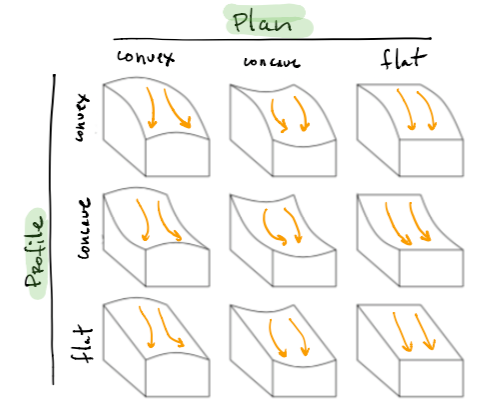
\includegraphics[width=0.9\linewidth]{figs/curvatures}
  \caption{Nine curvatures (Figure adapted from \citet{vanKreveld97}).}%
\label{fig:curvatures}
\end{figure}


%%%
\paragraph{Computing for grids.}
Computing the curvature is a complex operation and we will not describe one specific method.
The idea is to reconstruct \emph{locally} the surface (\eg\ with the polynomial fitting from Section~\ref{sec:polynomial} above, or with a TIN), and then verify whether the 2 curvature types are convex/concave/flat.
Observe that the curvature, as it is the case for the slope, is heavily influenced by the scale of the terrain (its resolution) and thus having a 3$\times$3 kernel might be influenced by the noise in the data, or by small features.


%%%
\paragraph{Computing for TINs.}
For a TIN, it is possible to define for each vertex $v$ the profile and the plan curvatures by using the triangles that are incident to $v$ and extract the contour line for the elevation of $v$ (as is shown in Figure~\ref{fig:saddle_contour}).
The idea is to classify each vertex into one of the 9 possibilities in Figure~\ref{fig:curvatures}.

If there is no contour segment, then $v$ is either a peak or a pit.
A peak will be profile and plan convex; a pit will be profile and plan concave.

If there are 2 segments, then we can use these to estimate the direction of the aspect, it will be perpendicular (thus the bisector between the 2 segments is a good estimate) in the direction or lower elevations.
If we simply look at the elevations higher and lower than $v$ along this direction, then we can easily verify whether $v$ is profile convex or concave.
For the plan curvature, we can simply walk along one of the 2 edges so that higher elevations are on our left, $v$ is plan convex if the contour line makes a left turn at $v$, if it makes a right turn it is concave, and if it is straight then it is plan flat.

If there are $>2$ segments, then $v$ is a saddle point and thus no curvatures can be defined.

%

When each point has been assigned a curvature---a pair $(profile,plan)$---we can use for instance the Voronoi diagram, as shown in Figure~\ref{fig:vd}.
\begin{marginfigure}
  \centering
  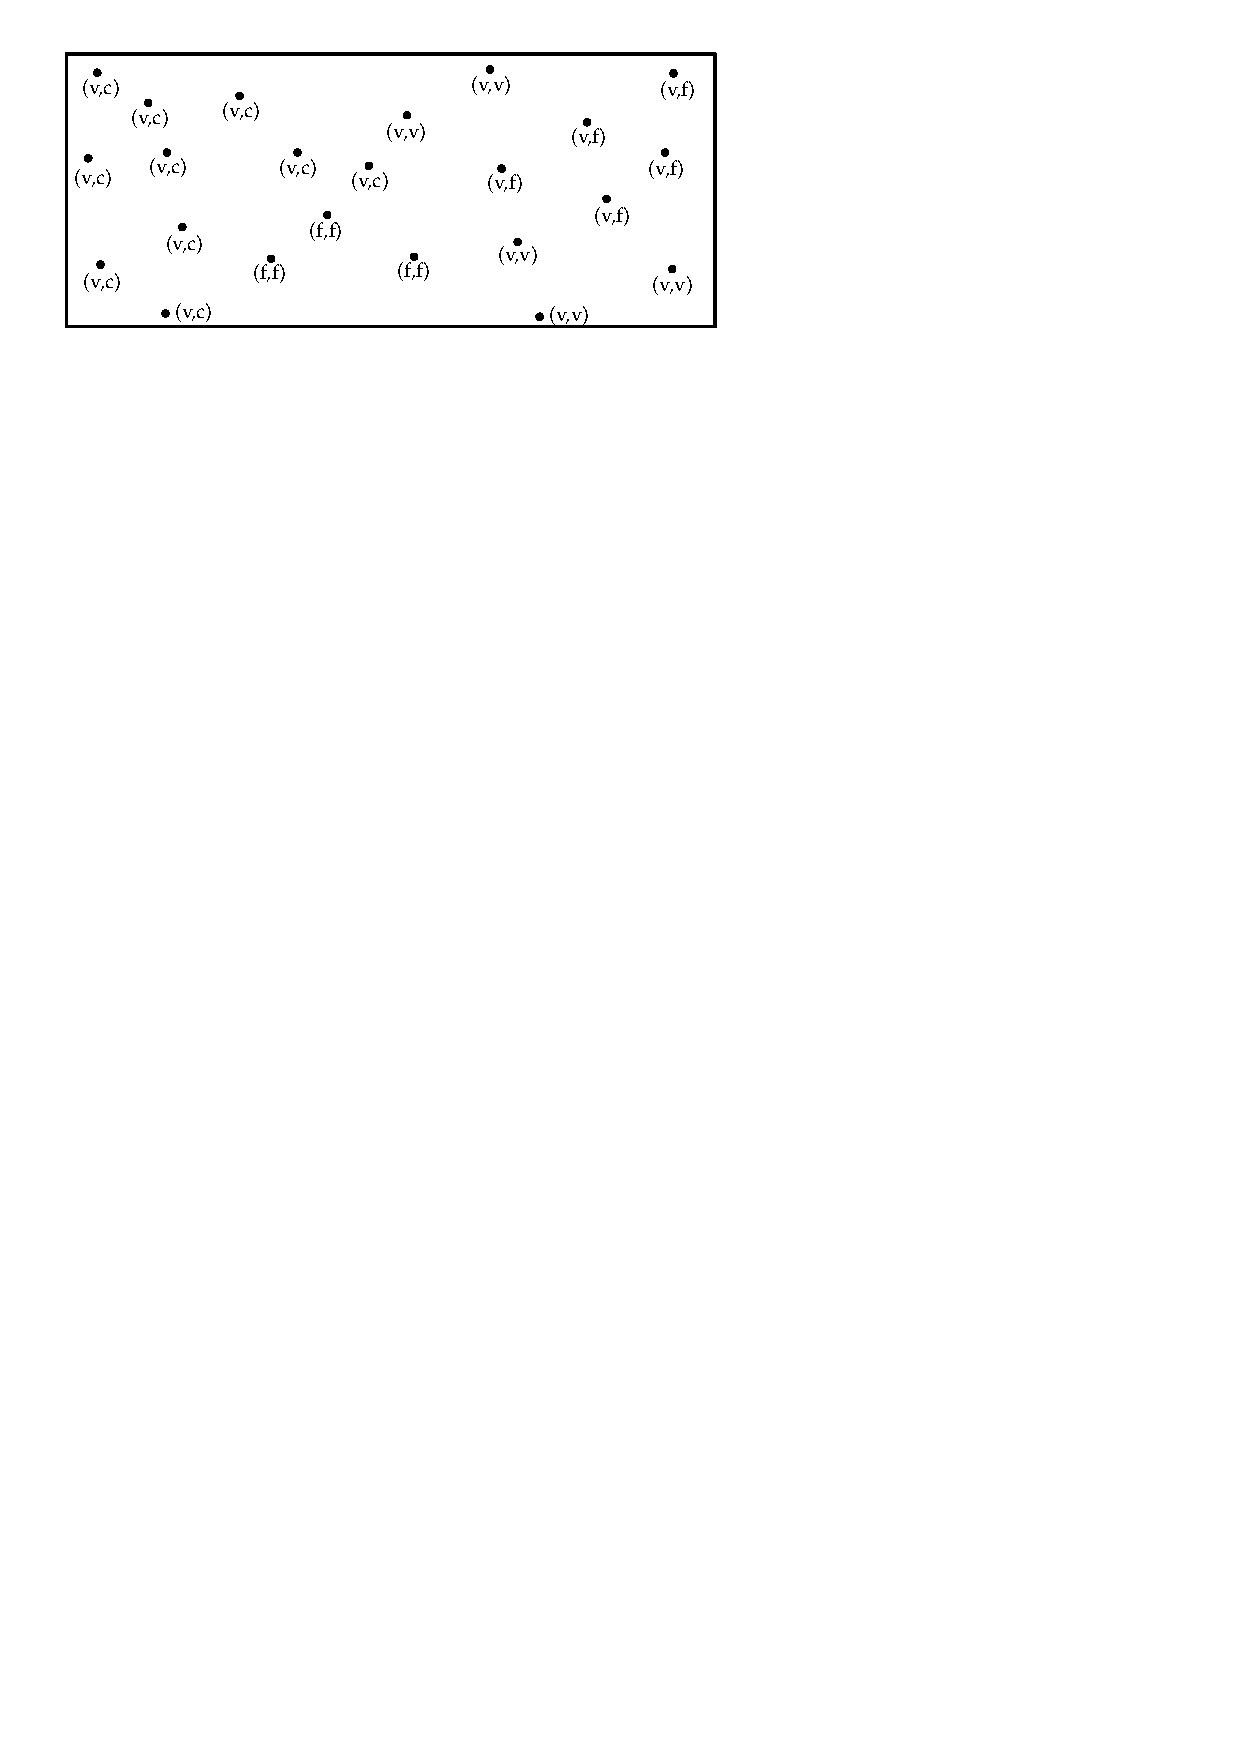
\includegraphics[page=1,width=\linewidth]{figs/vd}
  \includegraphics[page=2,width=\linewidth]{figs/vd}
  \includegraphics[page=3,width=\linewidth]{figs/vd}
  \caption{\textbf{(top)} Points from a TIN classified according to their curvatures (con\textbf{v}ex, con\textbf{c}ave, \textbf{f}lat). \textbf{(middle)} The VD of the points. \textbf{(bottom)} The Voronoi edges between the cells having the same label are removed, to create polygons.}%
\label{fig:vd}
\end{marginfigure}
It suffices to remove the Voronoi edges incident to cells having the same label, and polygonal zones are obtained.


%%%
%
\subsection{Roughness \& ruggedness}%
\index{roughness}\index{ruggedness}

The terms `roughness' and `ruggedness' are often used interchangeably and have slightly different definitions depending on the software and/or the documentation.
We can however claim that they both refer to how ``undulating'' or ``regular'' a (part of a) terrain is.
A terrain with a high roughness will have small local deviations, while one with low roughness will be ``smoother''.
In other words, the normals of the surface of the terrain will deviate from each others greatly for a high roughness, and less for low roughness.
Another way to measure roughness, is to think of it as the ratio between the surface area and its projection into a plane. 
\begin{marginfigure}
  \centering
  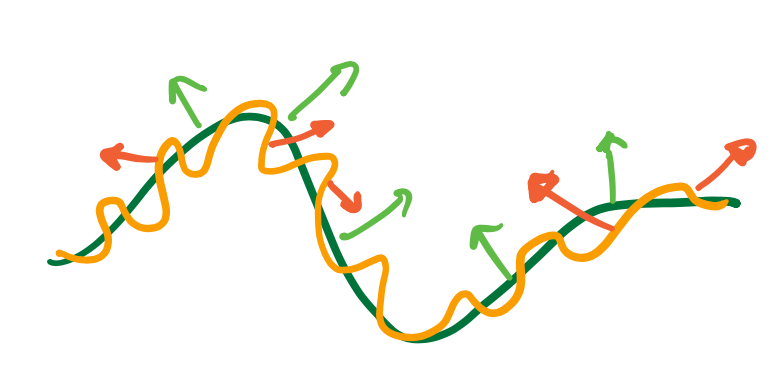
\includegraphics[width=\linewidth]{figs/roughness}
  \caption{The green profile of a terrain has a lower roughness than the orange one (normals locally deviate less).}%
\label{fig:roughness}
\end{marginfigure}

For gridded terrains, the roughness is most often calculated by simply looking at the differences in elevations for the cells inside a 3$\times$3 filter (or larger filter).
The roughness value for one location can be one of these variations (more exist):
\begin{itemize}
  \item the standard deviation of the 9 values (or 25 if a 5$\times$5 filter is used) in the filter;
  \item the largest difference in elevation between the value in the centre of the filter and one its neighbouring cell in the filter;
  \item the difference between the elevation of the central pixel and the mean of its surrounding cells;
\end{itemize}

It should be observed that these methods are highly influenced by the scale, \ie\ the resolution of the grid and the size of the filter will yield potentially very different results.

Notice also that since the differences in the elevations are used, a terrain that would be a constant slope (\eg\ a talus) would get a roughness that is not zero (in comparison to a perfectly flat terrain).
A solution to this would be to fit a plane with least-square adjustment to all the points involved in a filter, and then compare the differences of the elevations to plane.

%

For TINs, the same three variations above can be used for a single location ($x,y$), if for instance we pick the natural neighbours or if all the points within a certain distance threshold are used.
However, as mentioned above, how to create a new field of roughness is not as trivial as for a grid.
One could recreate a TIN with the values of the vertices having the roughness, or create a grid.




%%%
%
\section{Topographic features}

\begin{figure*}
  \centering
  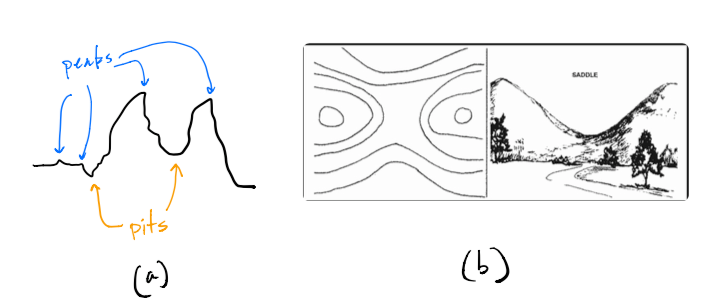
\includegraphics[width=\linewidth]{figs/feature_points}
  \caption{\textbf{(a)} Peaks and pits. \textbf{(b)} A saddle point (Figure from \url{https://www.armystudyguide.com})}%
\label{fig:feature_points}
\end{figure*}


%%%
\subsection{Peak}
A point $p$ whose surrounding is formed only of points that are of lower elevation is a peak.
The size and shape of the surrounding is dependent on the application and on the data model used to represent the terrain.
If a grid is used, this surrounding could be the 8 neighbours; if a TIN is used they could be the vertices that of the triangles incident to $p$.
Observe that a peak can be local,%
\marginnote{peaks and pits are local and influenced by the scale of the data}
that is one point that happens to be a few centimetres higher than all its neighbours would be classified as a peak (the small terrain in Figure~\ref{fig:feature_points} contains several peaks), while if we consider a hill we would surely consider only the top as the peak.
A peak is therefore on the scale of the data.

The contour line through the $p$ does not exist.

%%%
\subsection{Pit}
A point $p$ whose surrounding is formed only of points that are of higher elevation is a pit.
The same remarks as for peak apply here.
The contour line through the $p$ does not exist.

%%%
\subsection{Saddle point}%
\index{saddle point}

As shown in Figure~\ref{fig:feature_points}b, a saddle point, also called a pass, is a point whose neighbourhood is composed of higher elevations on two opposite directions, and 2 lower elevations in the other two directions.
From a mathematics point-of-view, it is a point for which the derivatives in orthogonal directions are 0, but the point is not maximum (peak) or a minimum (pit).

%

If we consider the contour line of a saddle point $p$, then there are 4 or more contour line segments meeting at $p$; for most point in a terrain this will be 2, except for peaks/pits where this is 0.
Figure~\ref{fig:saddle_contour}
\begin{marginfigure}
  \centering
  \includegraphics[page=2,width=\textwidth]{figs/saddle_contour}
  \caption{A saddle point at elevation \qty{10}{\m}, and its surrounding points. The triangulation of the area is created and used to extract the contour line segments at \qty{10}{\m} (red lines).}%
\label{fig:saddle_contour}
\end{marginfigure}
shows an example for a point with an elevation of \qty{10}{\m}, the contour lines at \qty{10}{\m} is drawn by linearly interpolating along the edges of the TIN of the surrounding (see Chapter~\ref{chap:conversion}).


%%%
\subsection{Valleys \& ridges}

\begin{figure}
  \centering
  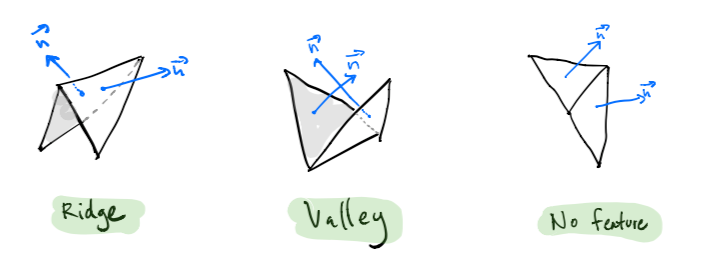
\includegraphics[width=\linewidth]{figs/valley_ridge}
  \caption{Edges in a TIN can be classified as valley, ridge, or neither}%
\label{fig:valley_ridge}
\end{figure}
Valleys and ridges are 1-dimensional features.
If a terrain is represented as a TIN, we can extract the edges of the triangles that form a valley or a ridge.
An edge $e$, incident to 2 triangles, is considered a valley-edge if the projection of the 2 normals of the triangles, projected to the $xy$-plane, point to $e$.
If the 2 normals projected point in the opposite direction, then $e$ is a ridge.
If they point is different directions, then $e$ is neither.



%%%
%
\section{Properties and features used in practice}[Properties used in practice]


%%%
\subsection{Slope}%

The slope (gradient + aspect) are a cornerstone of runoff modelling (see Chapter~\ref{chap:runoff}), the prediction of the flow and accumulation of water on a terrain.
The slope is used to calculate the flow direction at a given location, which is the direction with the steepest descent at that location.

%

The slope can also be used to predict the irradiation (from the sun) that a given location at a given day/time would receive.
This is often the input of (local) meteorological models, can be used to optimise the location of solar panels, to predict land surface temperature, 


%%%
\subsection{Curvature}%

While curvature is used implicitly to calculate the flow direction in runoff modelling, there are use-cases where the value is useful.
One of them is for the predicting of where snow covering will be.
% TODO: maybe a bit more about snow covering?

The values of the curvature can help a practitioners understand and characterise the drainage basins, once extracted from a terrain (see Section~\ref{sec:drainage_basins}).

% TODO: complete this section a bit? still a bit rough


%%%
\subsection{Roughness}%

The roughness can be used directly as a predictor for the habitats of different species.

The variations in roughness in a terrain can be used to delineate the terrain into geomorphological and geological areas.


%%%
\subsection{Hillshading}%
\index{hillshading}

Hillshading is a technique used to help visualise the relief of a gridded terrain (see Figure~\ref{fig:hillshade} for an example).
\begin{figure*}
  \centering
  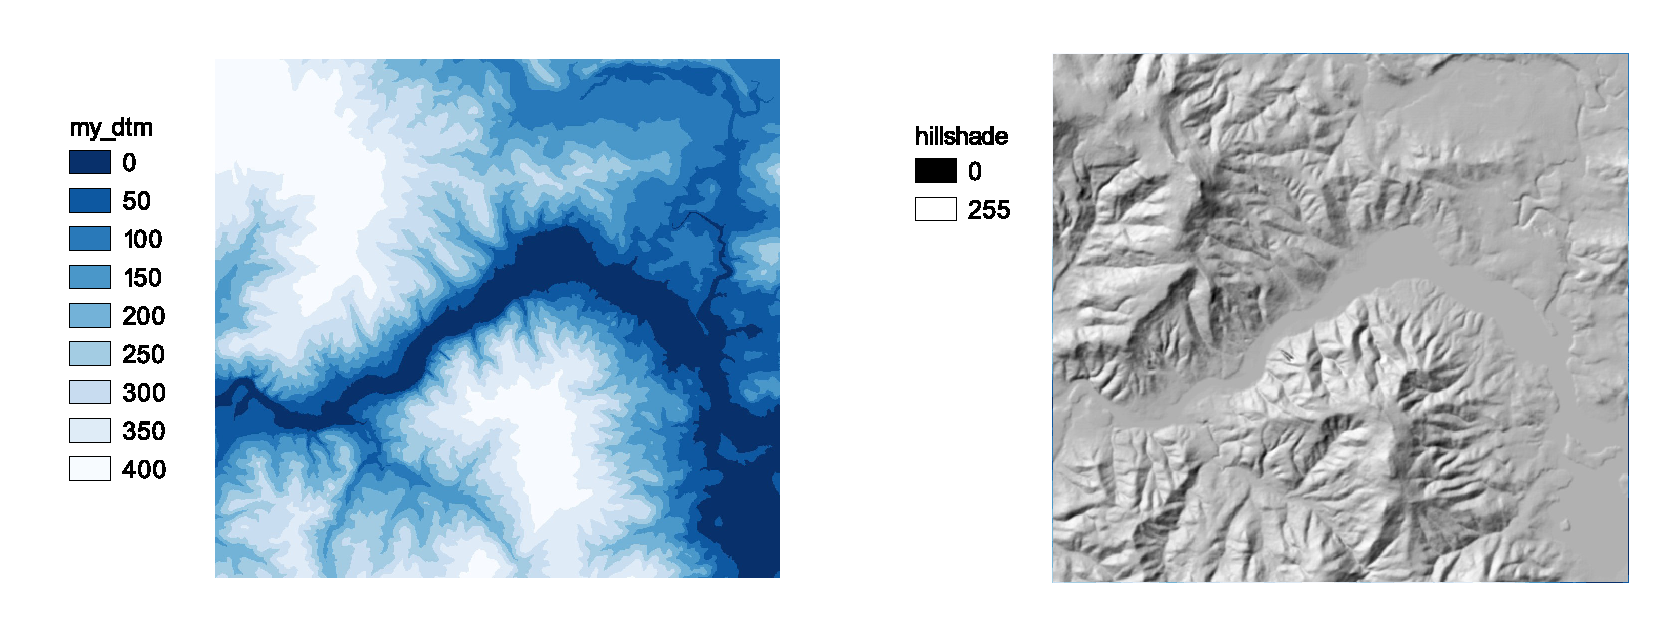
\includegraphics[width=\linewidth]{figs/hillshade}
  \caption{\textbf{Left}: a DTM visualised with height as a shade of blue. \textbf{Right}: when hillshading is applied.}%
\label{fig:hillshade}
\end{figure*}
It involves creating an image that depicts the relative slopes and highlights features such as ridges and valleys; a hillshade does not depict absolute elevation.
This image assumes that the source of light (the sun) is located at a given position (usually North-West).

\begin{floatbox}
  \begin{kaobox-practice}[frametitle=\faCog\ Why does the sunlight come from the North-West?]
    The source of the light for hillshading is usually set at the North-West, but in reality the sun is \emph{never} located there (in the northern hemisphere).
    Why is this a common practice then?
    The main reason is because the human brain usually assume that the light comes from above when looking at picture.
    Doing so reduces the chances of \emph{relief inversion}, \ie\ when mountains are perceived as valleys, and vice-versa.
    This \href{https://ramblemaps.com/why-does-sunlight-come-from-north}{website \faExternalLink} gives a clear example where a valley is interpreted as a mountain ridge by many if the sun is coming from the South.
  \end{kaobox-practice}
\end{floatbox}

While it would be possible to use advanced computer graphics methods (see Chapter~\ref{chap:visibility}) to compute the shadows created by the terrain surface, in practice most GIS implements a simplified version of it which can be computed very quickly.

Given a regular gridded terrain, hillshading means that each cell gets a value which depicts the variation in tone, from light to dark.
The output of a hillshade operation is thus a regular gridded DTM, usually with the same extent and resolution as the original grid (for convenience).
The values computed for each cell need as input the gradient and the aspect of the terrain\@.
The formula to compute the hillshade of a given cell $c_{ij}$ differs from software to software, and we present here one (it is used in ArcGIS for example, and surely others).
It assumes that the output hillshade value is an integer in the range $[0,255]$ (8-bit pixel), and that the direction (azimuth) and the height (given as an angle) of the illumination source is known.
Notice that the position of the sun is relative to the cell, its position thus changes for different cells of a terrain\@.
As above and in Figure~\ref{fig:hillshade-params}, 
\begin{figure}
  \centering
  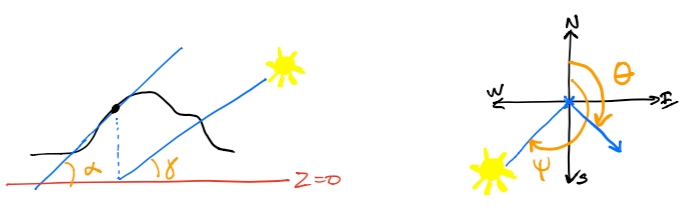
\includegraphics[width=0.95\linewidth]{figs/hillshade-params}
  \caption{The 4 parameters necessary to calculate the hillshade at a location (black point on the terrain).}%
\label{fig:hillshade-params}
\end{figure}
for a cell $c_{ij}$, its gradient is $\alpha_{ij}$, its aspect is $\theta_{ij}$, the azimuth of the sun is $\psi$ (angle clockwise from the north, like the aspect), and the height of the sun is $\gamma$ (0 rad is the horizon, $\frac{\pi}{2}$ rad is the zenith).
\begin{multline}  
  hillshade_{ij} = 255 \cdot \biggl[ \Big( \cos\left(\frac{\pi}{2} - \gamma\right) \cos(\alpha_{ij}) \Big) + \\
                         \Bigl( \sin\left(\frac{\pi}{2} - \gamma\right) \sin\left(\alpha_{ij}\right) \cos(\psi - \theta_{ij}) \Bigr) \biggr]
\end{multline}
Notice that: (1) all angles need to be radians; (2) if $hillshade_{ij} < 0$ then $hillshade_{ij} = 0$.


%%%
%
\section{Notes and comments}

The polynomial fitting method for computing the slope is from \citet{Evans80} and \citet{Wood96}.
\citet{Skidmore89} carried out a comparison of 6 methods to extract slope from regular gridded DTMs, and concluded that methods using 8 neighbours perform better than those using only 4 or the biggest height difference.
He did not however investigate how the resolution of the grid influences the results.

The formula to calculate the hillshade for one cell in a gridded DTM is from \citet{Burrough98}, and the ArcGIS manual describes it in details (\href{https://desktop.arcgis.com/en/arcmap/10.3/tools/spatial-analyst-toolbox/how-hillshade-works.htm}{link}).

Some algorithms have been developed to identify the features forming a DTM: \citet{Kweon94} and \citet{Schneider05} can identify simple features in DEMs (if they are pre-processed into bilinear patches); and \citet{Magillo09} and \citet{Edelsbrunner01-1} describe algorithms to perform the same, but directly on TINs.

The algorithm to extract profile and plan curvatures from a TIN is taken from \citet{vanKreveld97}.

\citet{Bohner09} give several concrete examples of the use of terrain properties for climatology applications, and provide details about one method to identify snow covering.

% A DTM is formed by an aggregation of many features that are inter-related~\citep{Pfalz76,Kweon94,DoD99,Wood96}.


%%%
%
\section{Exercises}

\begin{enumerate}
  \item What is the missing word? The \_\_\_\_\_\_\_\_\_ is the 2nd derivative of the surface representing the terrain, it represents the rate of change of the gradient.
  \item Given a raster, how to identify a valley and a ridge?
  \item If we want to compute the slope (gradient + aspect) for the cell at the centre of this 3$\times$3 DTM with the `finite difference method', what results will we get?
  \\
  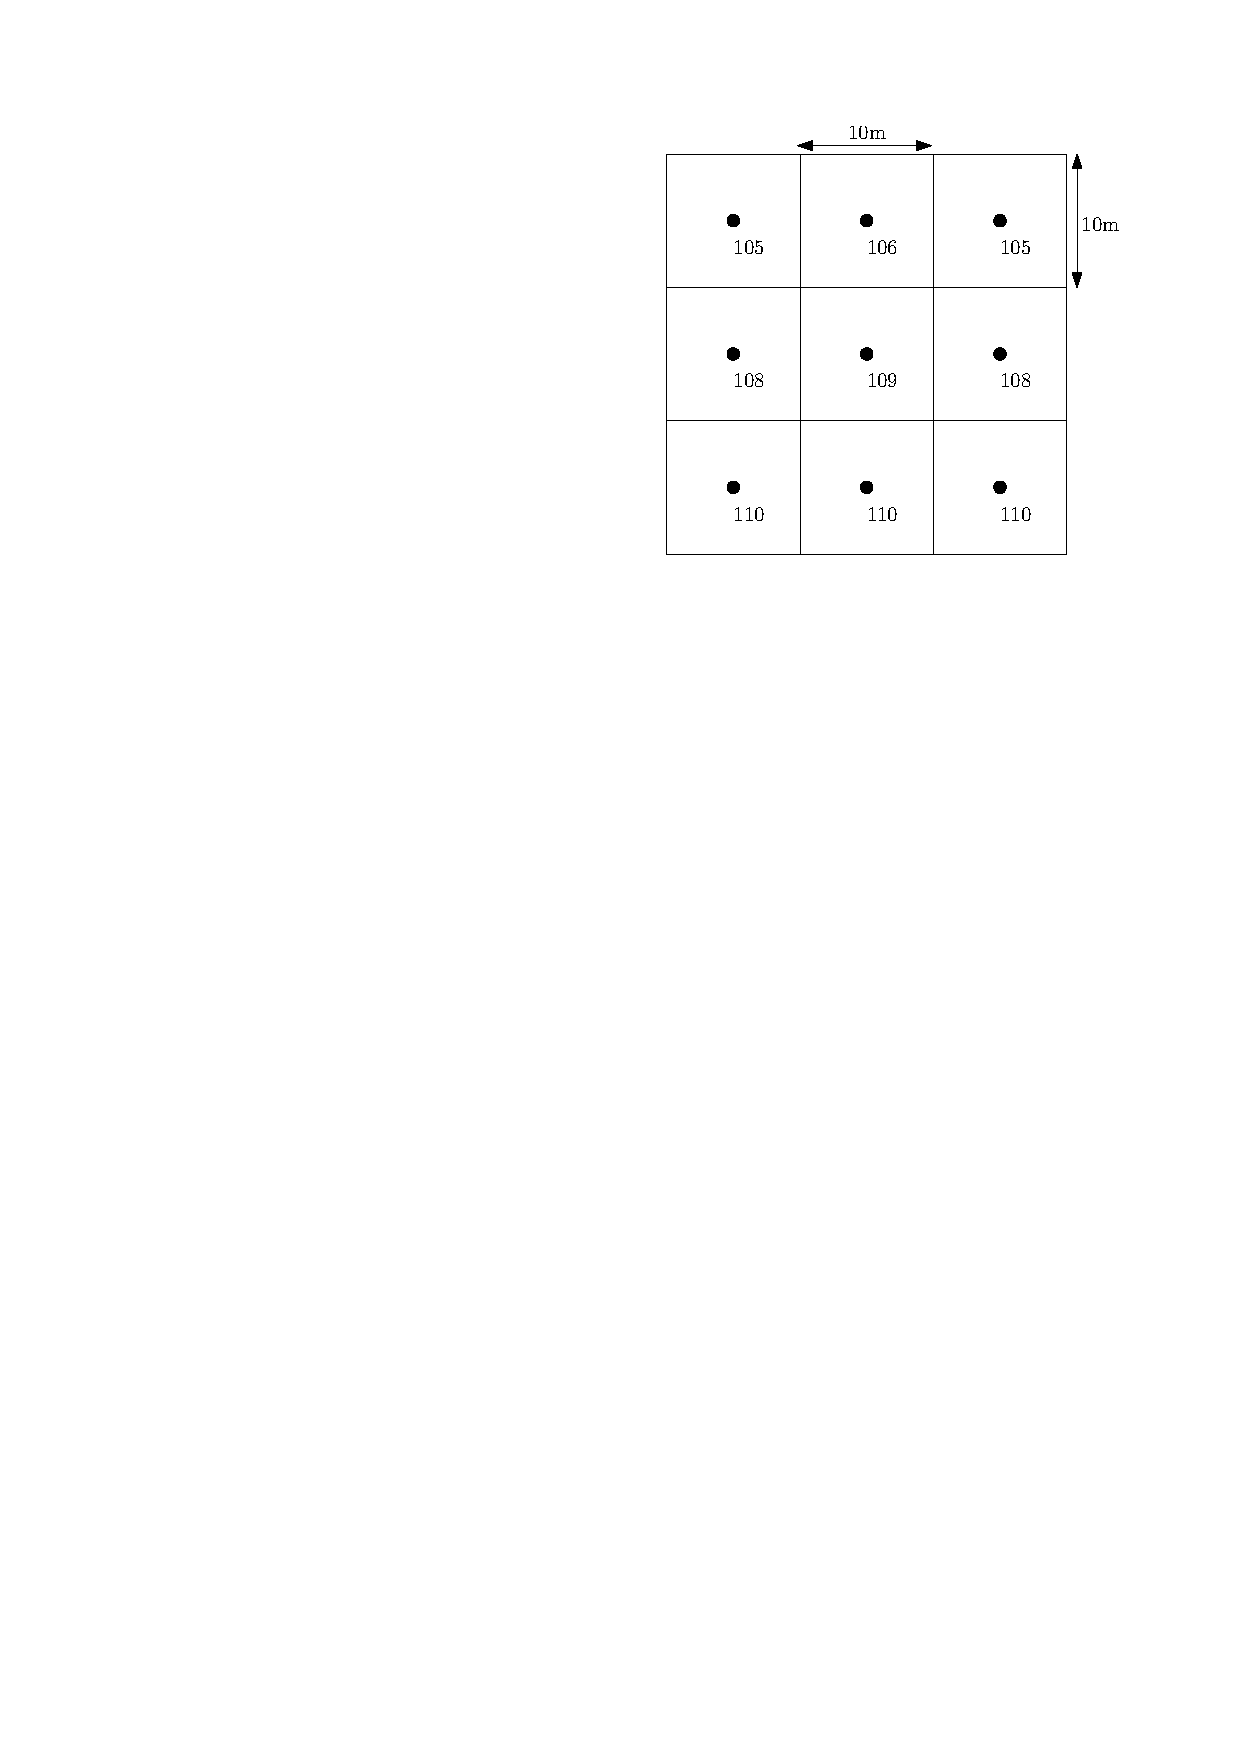
\includegraphics[width=0.4\linewidth]{figs/slope_grid_question}
\end{enumerate}
